\documentclass[../main.tex]{subfiles}
\begin{document}

\section{Synapses}
The second key element in neural circuits is the synapse.
Synapses serve as specialized intercellular junctions between neurons.
They are broadly categorized into two main types: \textbf{electrical synapses} and \textbf{chemical synapses}.

\textbf{Electrical synapses}, also known as gap junctions, establish a direct electrical connection between presynaptic and postsynaptic neurons through interlinking ion channels spanning both membranes.
In contrast, \textbf{chemical synapses} use neurotransmitters as secondary messengers to transmit the presynaptic signal.
The introduction of a secondary messenger enhances the computational power of chemical synapses, enabling various forms of gain control, plasticity, and inhibitory shunting.
% This increased computational capacity is reflected in the diversity of molecular components, such as neurotransmitters, postsynaptic receptors, and presynaptic receptors.
The structural arrangement of chemical synapses varies greatly, encompassing factors like the number and size of presynaptic vesicles, active zones, postsynaptic densities, and postsynaptic receptors.
\begin{figure}[t]
    \centering
    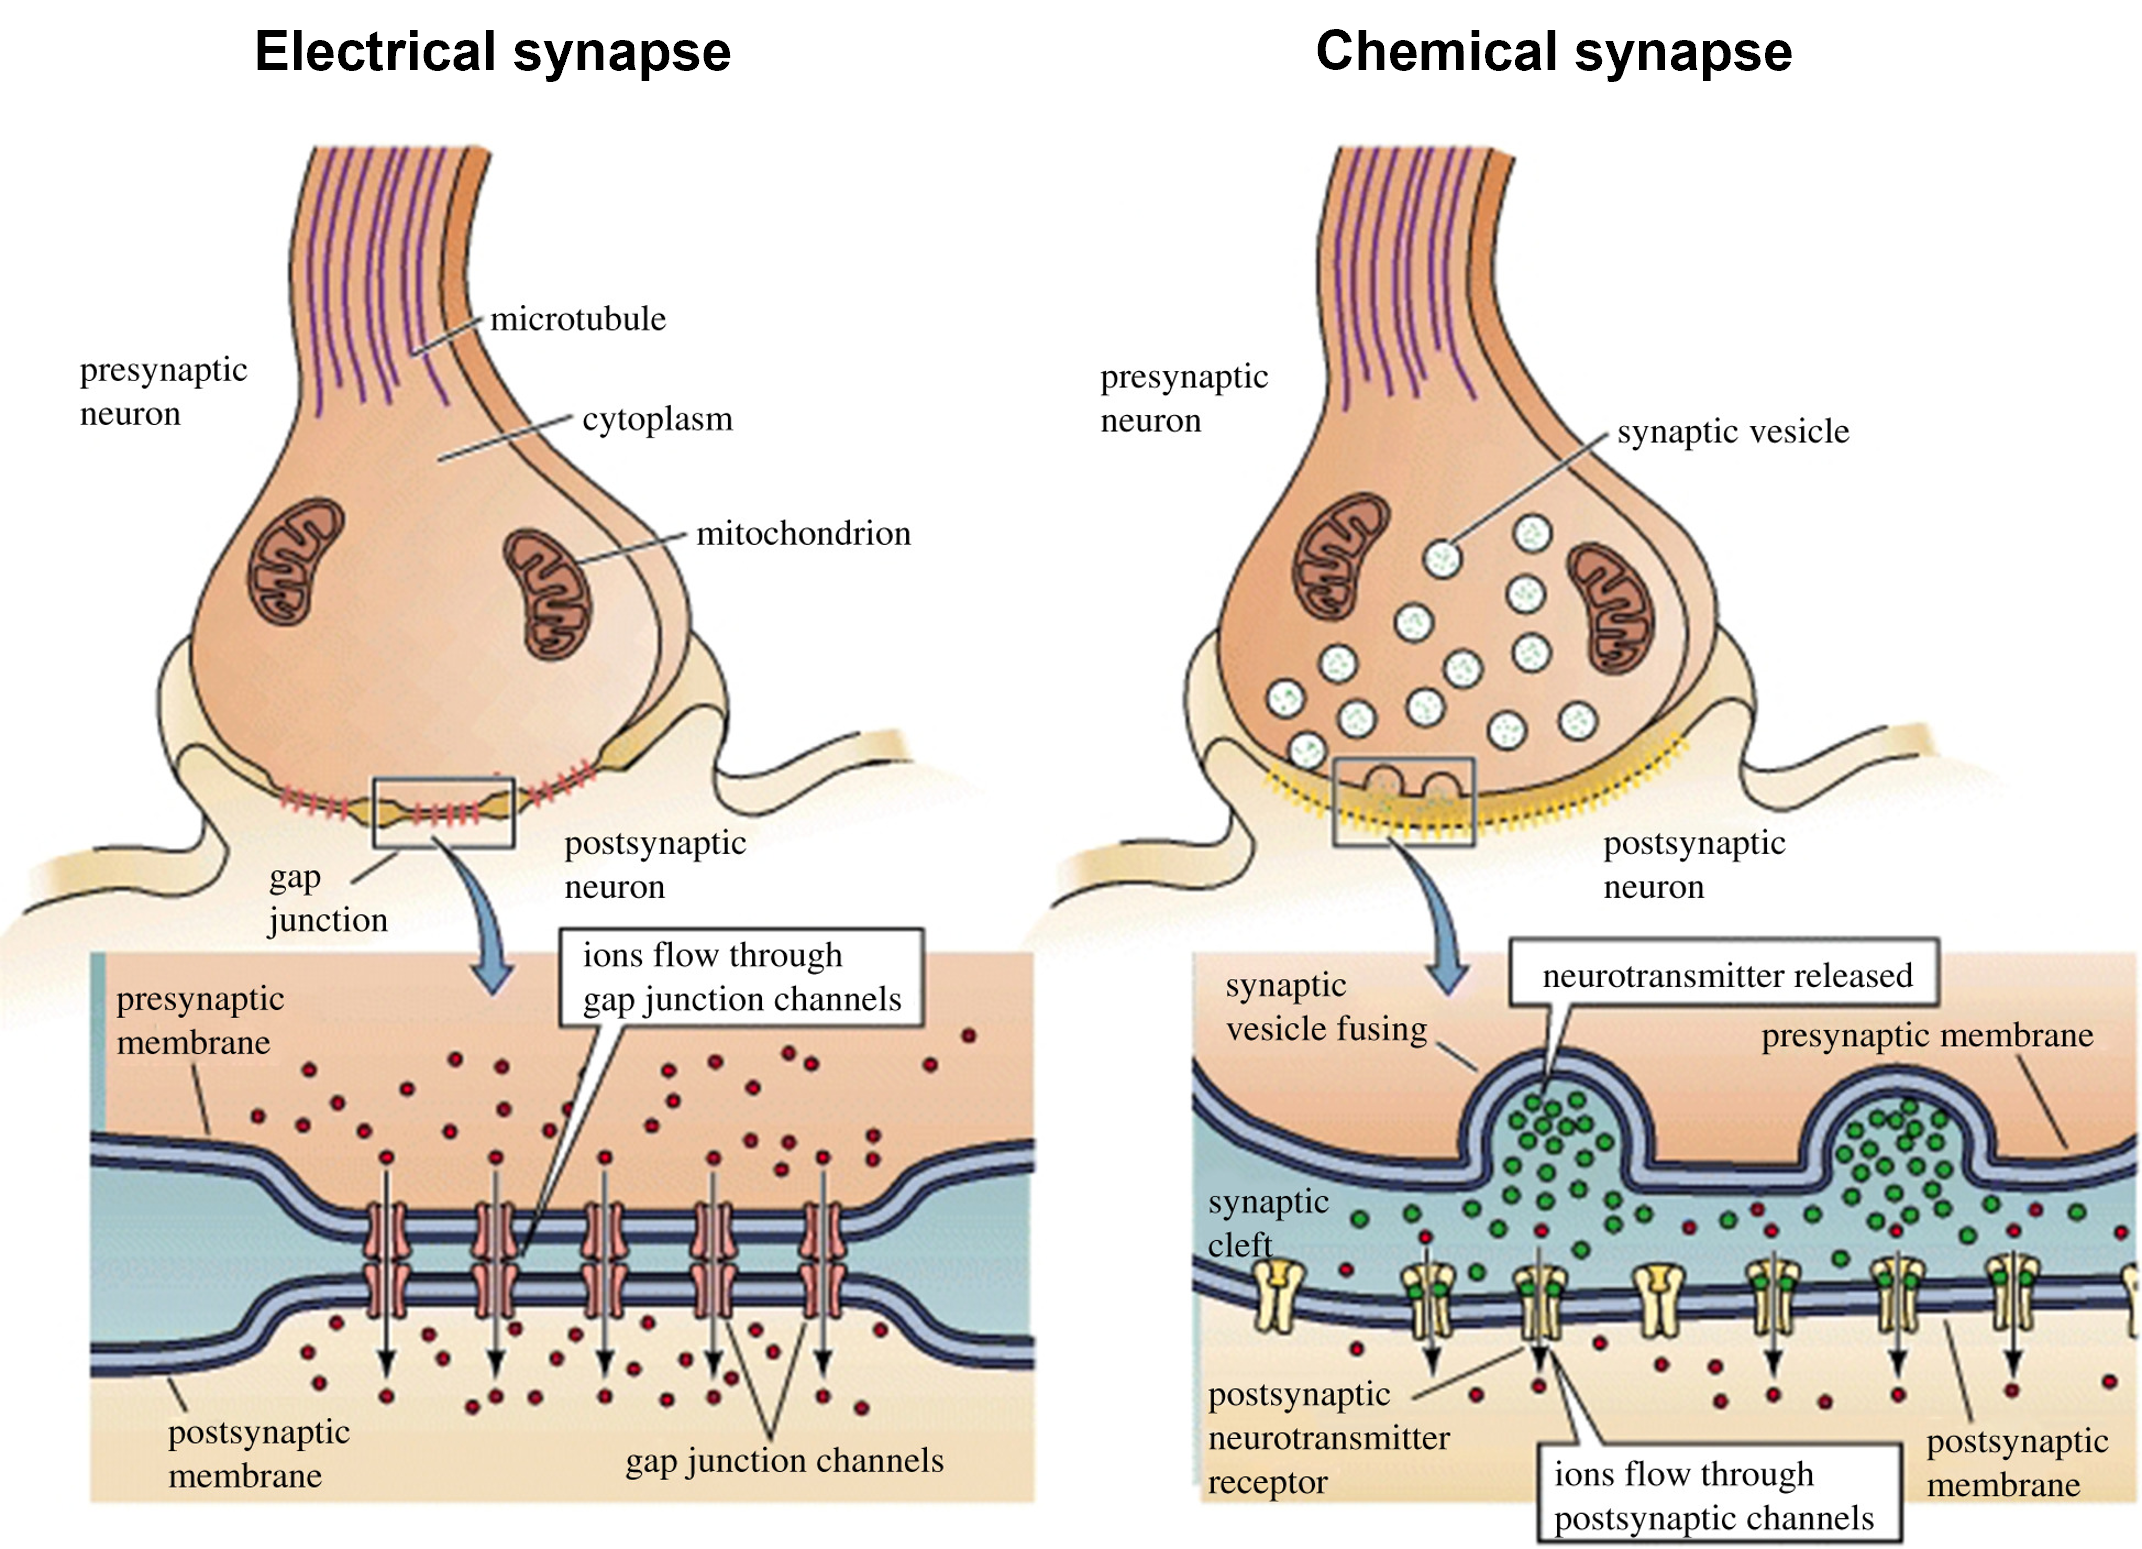
\includegraphics[width=\textwidth]{chapter1/figures/synapses.png}
    \caption{\textbf{Chemical synapses and electrical gap junctions}.
    Electrical synapse is mediated by intercellular channels known as gap junctions, which provide a pathway for spreading electrical currents between adjacent cells (left).
    Chemical synapse is one-directional and mediated by the release of neurotransmitters contained at the presynaptic vesicles, that bind to specific receptors in the postsynaptic cell (right).
    Original figure from \cite{towlson2018caenorhabditis}.}
   \label{fig:synapses_schematics}
\end{figure}
Figure \ref{fig:synapses_schematics} illustrates schematics of these two types of synapses.

The basic events of chemical synaptic transmission can be sequenced as follows:
\begin{enumerate}
    \item An action potential arrives at the presynaptic terminal, depolarizing the membrane.
    \item Depolarization triggers the opening of voltage-dependent $\text{Ca}^{2+}$ channels, leading to a transient increase in intracellular ionic calcium concentration, [Ca$^{2+}]_i$.
    \item The rise in [Ca$^{2+}]_i$ increases the probability of one or more synaptic vesicles fusing with the presynaptic membrane, releasing neurotransmitters into the synaptic cleft.
    \item Neurotransmitters diffuse across the synaptic cleft.
    \item Neurotransmitters bind to postsynaptic receptors, inducing a conformational change in the receptors.
    \item Depending on the nature of the receptor, ionotropic or metabotropic, the subsequent step varies.
    For ionotropic receptors, the conformational change opens their internal ion channels, allowing the flow of ionic currents.
    This results in \textbf{either an excitatory postsynaptic current} (EPSC) or an \textbf{inhibitory postsynaptic current} (IPSC) depending on the channels that were opened.
    For metabotropic receptors, the conformational change initiates a series of intracellular reactions that produce a desired end effect, such as enzyme phosphorylation or upregulation of a specific receptor subunit.
\end{enumerate}

The neurotransmitters synthesized and released form the basis for the classification of neurons as excitatory or inhibitory. 
Glutamatergic neurons, such as AMPAergic neurons ($\alpha$-amino-3-hydroxy-5-methyl-4-isoxazolepropionic acid) or NMDAergic neurons (N-methyl-D-aspartate), release glutamate, exciting postsynaptic cells. 
GABAergic neurons, on the other hand, release GABA ($\gamma$-aminobutyric acid), which inhibits postsynaptic neurons.
The delicate balance between excitation and inhibition is crucial for the precise functioning of the nervous system.
Perturbations in this balance have been associated with various disorders, including epilepsy, autism, and mental retardation \cite{villa_excitatory_2016}.
\subsection{Modelling synapses}
Modelling synaptic transmission involves capturing the underlying biophysical processes described previously.
As synapses exhibit changes in their properties across various time scales, synaptic transmission is inherently a highly dynamic process.

In the context of large-scale neural networks, incorporating a high level of detail and complexity into the synaptic dynamics can significantly increase computational costs.
Consequently, certain assumptions are necessary to strike an appropriate balance between biological plausibility and computational efficiency.

Several simple models have been proposed to successfully capture both the time and voltage dependence of synaptic transmission. 
In general, within the conductance-based model, the postsynaptic current can be described as follows:
\begin{equation}
    I_{\text{syn}} = g_{\text{syn}}(t,v)(v-E_{\text{syn}}),
    \label{eq:synaptic-current}
\end{equation}
where the subindex syn refers to the synapse and the term $E_{\text{syn}}$ indicates the reversal potential of the synaptic conductance, which determines whether the synapse tends to depolarize (excitatory) or to hyperpolarize (inhibitory) the membrane.
Typical values for E$_{\text{syn}}$ are around $0$ and $-75$ mV for excitatory and inhibitory synapses, respectively. 
The conductance $g_{\text{syn}}$ remains zero until the arrival of a presynaptic action potential. 
This term depends on both the time and the voltage of the postsynaptic neuron. For simplicity, it can be considered separable.
Thus, the conductance can be expressed as:
\begin{equation}
    g_{\text{syn}}(t, v) = g_{\text{max}} a(t)b(v),
    \label{eq:synaptic-conductance}
\end{equation}
where $a(t)$ determines the time dynamics and $b(v)$ represents voltage-dependency.
Both functions $a(t)$ and $b(v)$ are normalized to ensure that $g_{\text{max}}$ determines the maximum value of $g_{\text{syn}}$.

\subsubsection{Time-dependency}
Several functions $a(t)$ have been proposed to describe the temporal dynamics of the postsynaptic currents.
One of the most common is the exponential decay function:
\begin{equation}
    a(t) = \exp{\bigg(-\displaystyle\frac{t-t_s}{\tau_d}}\bigg), \hspace{2mm} t \ge t_s,
    \label{eq:1-exp-syn}
\end{equation}
but the double exponential function is also commonly used:
\begin{equation}
    a(t) = \displaystyle\frac{1}{a_{\text{max}}}\Bigg[ 
    \exp{\bigg( -\displaystyle\frac{t-t_s}{\tau_d}\bigg)}
    -     \exp{\bigg( -\displaystyle\frac{t-t_s}{\tau_r}\bigg)}
    \Bigg], \hspace{2mm} t \ge t_s,
    \label{eq:2-exp-syn}
\end{equation}
where $a_{\text{max}}$ is a normalization constant, and $\tau_d$ and $\tau_r$ are the decay and rise time constants. 
The main difference between these descriptions is that the exponential decay function \eqref{eq:1-exp-syn} does not consider the rising dynamic of the conductance.
Consequently, the conductance rises instantaneously from $0$ to $1$ at $t=t_s$, where $t_s$ represents the time of the synaptic action potential arrival.
The double exponential function \eqref{eq:2-exp-syn} offers a better approach, as it incorporates a finite rise time.

However, these approaches have limitations.
In some cases, the decay of synaptic conductance is characterized by several time constants, as seen in the conductance of NMDA receptors.
Conversely, the fast AMPA receptor conductance exhibits sigmoidal activation.
For this reason, a multi exponential function can be useful for modelling these time dynamics:
\clearpage
\begin{equation}
    a(t) = \displaystyle\frac{1}{a_{\text{max}}}
    \Bigg[1-\exp{\bigg(-\displaystyle\frac{t-t_s}{\tau_\alpha}\bigg) }\Bigg]^{n}
    \Bigg[ \displaystyle\sum_{i=1}^{m} a_i\exp{\bigg(-\displaystyle\frac{t-t_s}{\tau_{d,i}} \bigg)} \Bigg], \hspace{2mm} t \ge t_s.
    \label{eq:multiexp-syn}
\end{equation}
When the term $n>1$, the function denotes a sigmoidal response of the synaptic activation.
The set $\{\tau_{d,i}\}_{i=1}^{m}$ represents multiple ($m$) decay time constants describing the decline of the function $a(t)$. 
This model has the advantage of reproducing a more realistic activation pattern, albeit with an increase in computational cost.
This makes it a non-optimal choice for large-scale network modelling. 

Another popular expression for $a(t)$ is the so-called alpha function: 
\begin{equation}
    a(t) = \displaystyle\frac{t-t_s}{\tau_\alpha}\exp{\bigg(1-\displaystyle\frac{t-t_s}{\tau_\alpha}\bigg)}, \hspace{2mm} t \ge t_s,
    \label{eq:alpha-syn}
\end{equation}
where $\tau_\alpha$ represents the time where $a(t)$ reaches its maximum value. 
As difference of the double exponential synaptic model \eqref{eq:2-exp-syn} $\tau_r$ and $\tau_d$ are constrained to be equal, $\tau_\alpha$ = $\tau_r$ = $\tau_d$. 
This function effectively characterizes synaptic conductances with similar rise and decay times.
Figure \ref{fig:a-functions} compares the time evolution of $a(t)$ considering single exponential, double exponential, and alpha functions.
\begin{figure}[!htb]
    \centering
    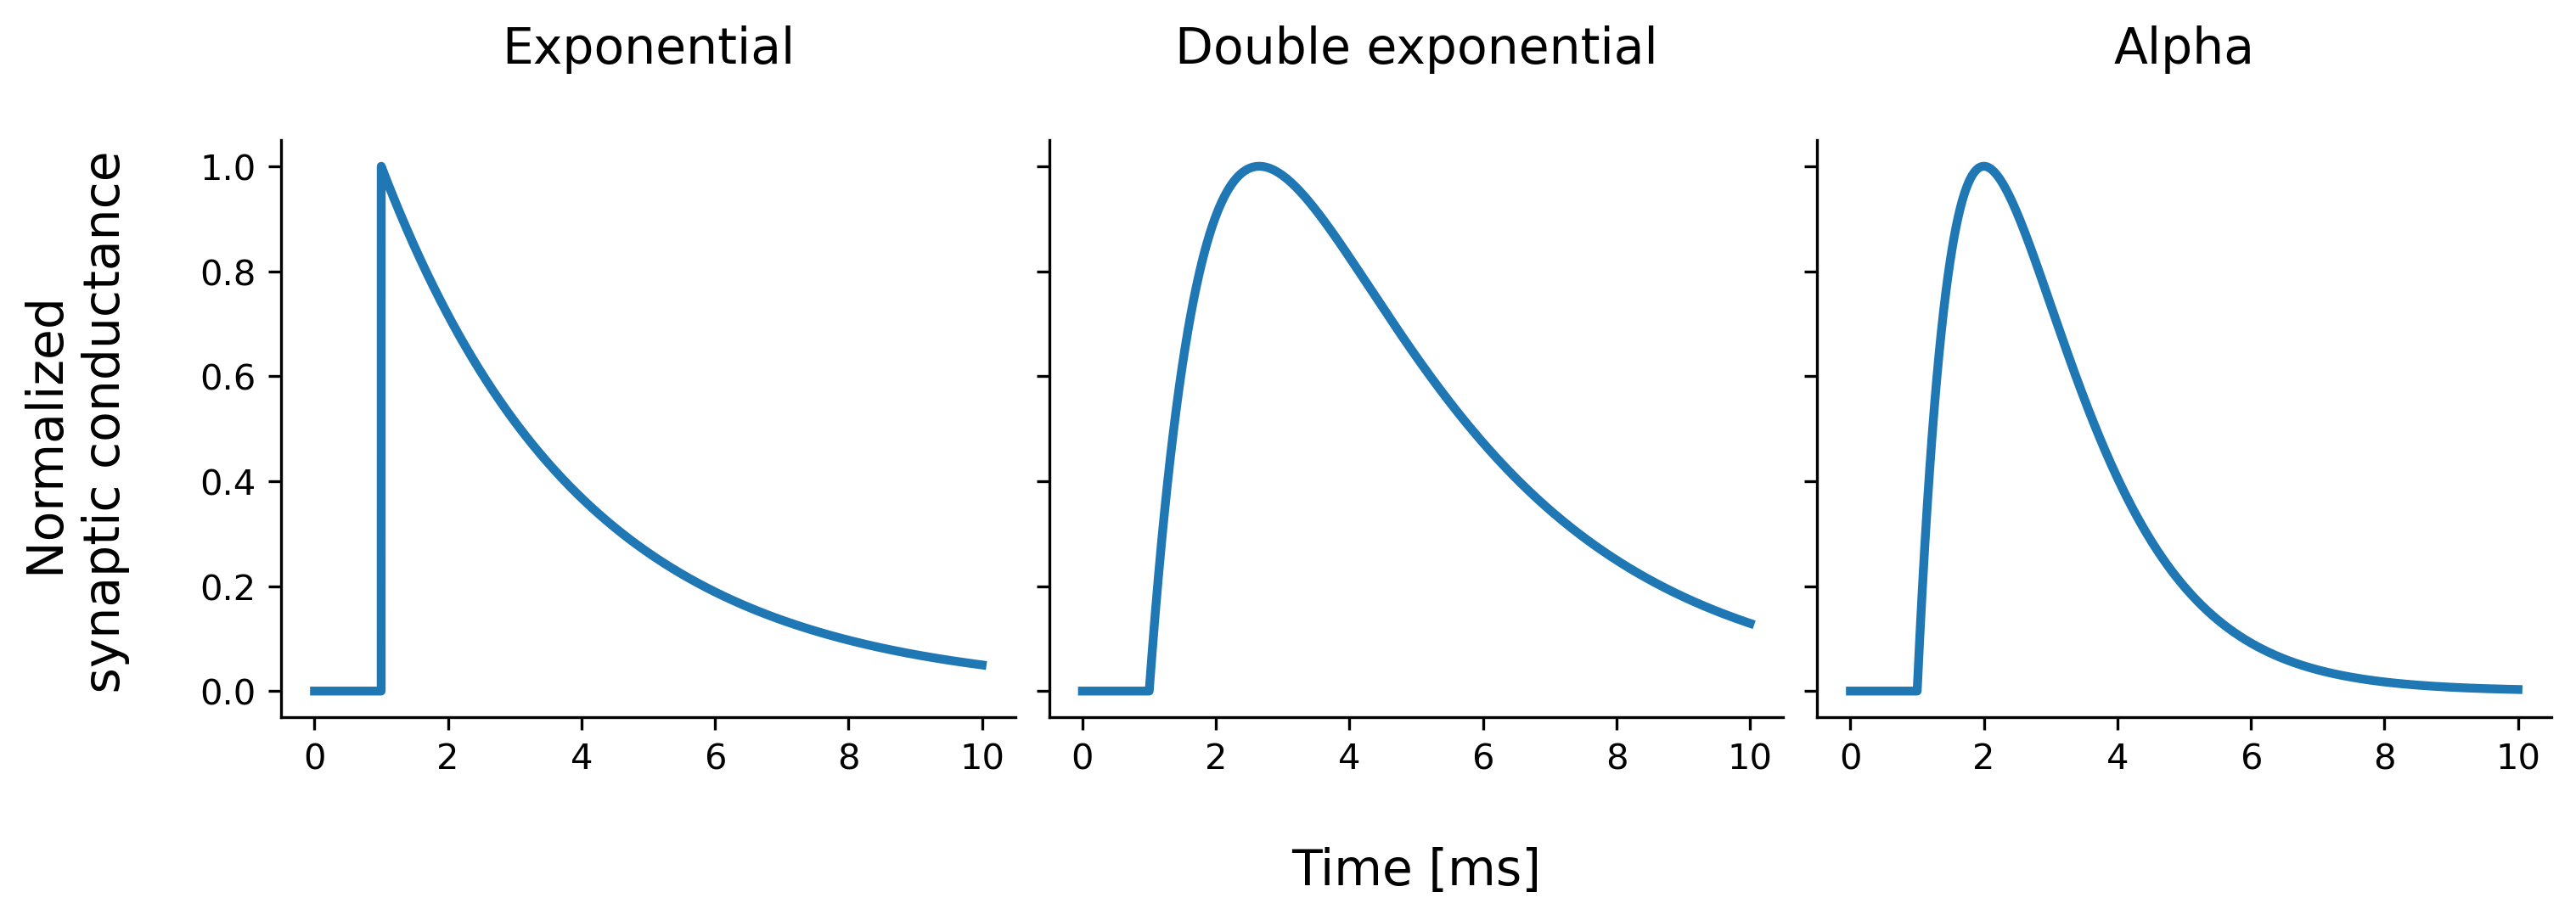
\includegraphics[width=\textwidth]{chapter1/figures/synaptic_conductances.png}
    \caption{\textbf{Different synaptic conductance modelling}.
    Evolution time of the synaptic conductance $g_\text{syn}$ for the single exponential decay function ($\tau$ = 3 ms), the double exponential function ($\tau_r$ = 3 ms and $\tau_d$ = 1 ms) and the alpha function ($\tau_\alpha$ = 1 ms).}
    \label{fig:a-functions}
\end{figure}
% \clearpage
\subsubsection{Voltage dependence of the synapse}
Most ligand-gated ion channels involved in synaptic transmission, such as AMPA or GABA$_\text{A}$ receptors, typically exhibit an approximately linear current-voltage relationship when open, and thus, $b(v) \approx 1$. 
However, excitatory synaptic currents often involve both AMPA and NMDA components, each activated by glutamate but with different sensitivities.
The general linear dependence observed in AMPA synapses does not apply to NMDA synapses. 
This non-linearity arises due to the blockage of the NMDA receptor pore from the extracellular side by a positively charged magnesium ion.
To account for this magnesium blocking phenomenon, the most commonly used expression for $b(v)$ is described as \cite{jahr_voltage_1990}:
\begin{equation}
    b(v) = \Bigg[1 + \displaystyle\frac{e^{-av}[\text{Mg}^{2+}]_o}{b}\Bigg]^{-1},
    \label{eq:mgblock-syn}
\end{equation}
where $[\text{Mg}^{2+}]_o$ is the extracellular magnesium concentration, usually 1 mM, and $a$ = 0.062 mV$^{-1}$ and $b$ = 3.57 mM. 

% Additionally, Ca$^{2+}$ plays and important role in intracellular signaling, and sometimes it is necessary to include ion calcium dynamics in a synaptic model.
% \textbf{ meter aqui lo del calcium dynamics si finalmente corresponde con lo de las neuronas cck y tal.}

% \subsection*{Stochasticity}
% All the previous description \eqref{eq:synaptic-current}-\eqref{eq:mgblock-syn} is completely deterministic: under the same conditions, the model's postsynaptic response is identical in size and shape on the arrival of a presynaptic action potential. 
% It is well known, that real synapses exhibit trial-to-trial variability.
% Sometimes, the addition of some kind of stochasticity into a synaptic model can be necessary \textbf{CITA}

% \subsection*{Plasticity}
% Not to sure of commenting this as well. 
% We don't use plasticity in this thesis, but maybe is important to comment, with the correspondent
\end{document}

Esto no toca aqui. Pero de un paper reciente sabemos que la granger casuality no está diseñada para point-processes series, 
se ha in tentado crear series contínuas através de filtros o kernel suavizadores, pero esto puede generar resultados 
espúreos. Se han intentado méotodos alternativos para poder aplicarlos a spikes trines. Analyzing multiple spike trains with nonparametric
granger causality